% Publication figure generated from the completed 4/2/1-mm
% crack-increment sensitivity study.
%
% MATLAB source:
%   verification/crack_path/plot_increment_sensitivity_coarse_publication.m
%
% Generated vector panels:
%   trajectory.pdf
%   vertical_deviation.pdf
%   direction_deviation.pdf
%   turn_density.pdf

\begin{figure}[tbp]
  \centering

  \begin{subfigure}[t]{0.485\linewidth}
    \centering
    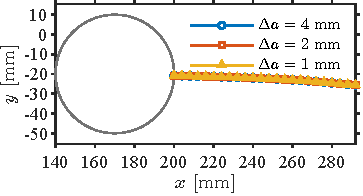
\includegraphics[width=\linewidth]{figures/increment_sensitivity/trajectory.pdf}
    \caption{Independently propagated crack trajectories for
    $\Delta a=4$, 2, and 1 mm, all continued to 92 mm.}
    \label{fig:inc-trajectory}
  \end{subfigure}
  \hfill
  \begin{subfigure}[t]{0.485\linewidth}
    \centering
    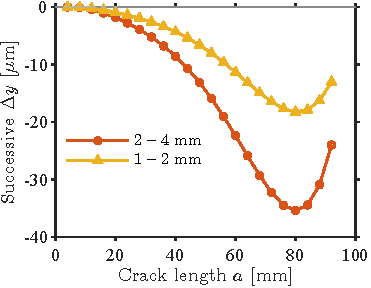
\includegraphics[width=\linewidth]{figures/increment_sensitivity/vertical_deviation.pdf}
    \caption{Successive vertical-coordinate differences,
    $y_{2\,\mathrm{mm}}-y_{4\,\mathrm{mm}}$ and
    $y_{1\,\mathrm{mm}}-y_{2\,\mathrm{mm}}$, evaluated at exact
    common crack lengths.}
    \label{fig:inc-dy}
  \end{subfigure}

  \medskip

  \begin{subfigure}[t]{0.485\linewidth}
    \centering
    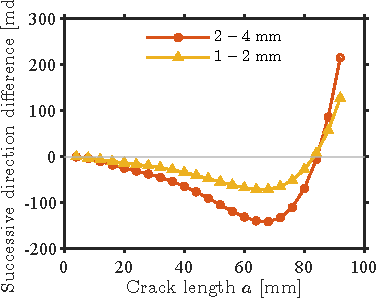
\includegraphics[width=\linewidth]{figures/increment_sensitivity/direction_deviation.pdf}
    \caption{Successive differences in absolute crack direction in the
    frozen initiation frame.}
    \label{fig:inc-dtheta}
  \end{subfigure}
  \hfill
  \begin{subfigure}[t]{0.485\linewidth}
    \centering
    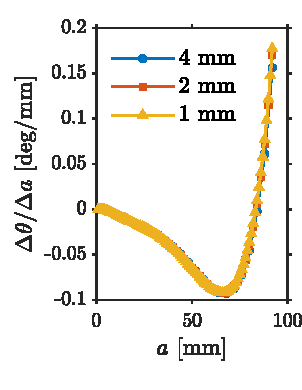
\includegraphics[width=\linewidth]{figures/increment_sensitivity/turn_density.pdf}
    \caption{Turning density $\Delta\theta/\Delta a$ along the three
    independently propagated trajectories.}
    \label{fig:inc-turn-density}
  \end{subfigure}

  \caption{Crack-increment sensitivity of the independently propagated
  LEFM paths. All three calculations use the same dimensionless coarse
  numerical family, with the absolute core, interaction-domain, transition,
  and exterior length scales reduced together with $\Delta a$. The
  trajectory panel shows the actual paths, while the two difference panels
  resolve successive changes at exact common crack lengths. The turning-
  density panel is plotted on each level's native crack-length grid.}
  \label{fig:increment-sensitivity}
\end{figure}
